% ============================================================================
%  Benchmarking salarial para Ecuador
%  Maestria en Inteligencia Artificial - USFQ
%
%  COMPILAR:  pdflatex tesis.tex  (dos veces, para el indice y las referencias)
%
%  Este documento se redacta a partir de `docs/registro_decisiones.md` (D-001 a
%  D-031) y `docs/mediciones.md`. Toda cifra citada aqui tiene su script y su
%  salida en `research/experimentos/`. Las referencias marcadas con [VERIFICAR]
%  necesitan que se confirme la paginacion antes de la entrega.
% ============================================================================
\documentclass[12pt,a4paper]{report}

\usepackage[utf8]{inputenc}
\usepackage[T1]{fontenc}
\usepackage[spanish,es-tabla]{babel}
\usepackage{amsmath,amssymb}
\usepackage{booktabs}
\usepackage{graphicx}
\usepackage{longtable}
\usepackage[margin=3cm]{geometry}
\usepackage{microtype}
\usepackage[hidelinks]{hyperref}
\usepackage{enumitem}
\usepackage{caption}
\graphicspath{{figuras/}}

\newcommand{\dref}[1]{\textbf{D-#1}}
\newcommand{\cargo}[1]{\texttt{#1}}

\title{\bfseries Benchmarking salarial con etiquetas de puesto delgadas:\\
       cuanto error es reducible por elegir mejor el grupo de comparacion}
\author{Pablo Andres Encalada}
\date{Maestria en Inteligencia Artificial --- USFQ\\[1ex]\today}

\begin{document}
\maketitle

% ============================================================================
\chapter*{Resumen}
\addcontentsline{toc}{chapter}{Resumen}

Un benchmark salarial responde a una pregunta simple: \emph{cuanto paga el mercado
por este puesto}. La dificultad no esta en el calculo sino en el denominador ---
que puestos se consideran comparables. Este trabajo parte de un catalogo real de
nominas ecuatorianas donde la etiqueta de cargo es texto libre, y mide cuanto del
error de un benchmark es reducible eligiendo mejor el grupo de comparacion.

La contribucion principal no es un algoritmo. Es una \textbf{medicion del
presupuesto disponible}: se descompone el error de prediccion en la parte
irreducible ---la que genera el empleador--- y la parte atribuible a agrupar mal,
y se establece que el techo de mejora por agrupacion es del orden del 12\,\%.
Sobre ese techo se construye un estimador y se mide cuanto de el se recupera.

El trabajo incluye un resultado negativo en el centro: la hipotesis con la que
arranco el proyecto ---que la composicion del pago (fijo, comisiones, extras)
discrimina puestos--- se midio y quedo en un $R^2$ fuera de muestra de $+0{,}0042$
contra un placebo en $-0{,}0002$. El eje que si paga resulto ser el \emph{nivel
jerarquico}, con $\omega^2 = 0{,}2462$ y un recorrido salarial de $2{,}11\times$
entre el escalon mas bajo y el mas alto. Ese giro, y el protocolo que lo hizo
visible, son parte del aporte.

\tableofcontents

% ============================================================================
\chapter{El problema}

\section{Que es un benchmark salarial y por que es dificil}

Una empresa que quiere saber si paga bien necesita comparar el sueldo de cada
persona contra lo que el mercado paga por \emph{ese mismo puesto}. El calculo es
trivial: una mediana. La dificultad esta enteramente en decidir que observaciones
entran en ella.

La industria resuelve esto con taxonomias duras: catalogos cerrados de puestos a
los que el cliente mapea su nomina a mano. Ese mapeo es caro, es lento, y es
donde se pierde la informacion --- dos empresas mapean el mismo puesto a
categorias distintas segun quien haga el ejercicio.

La alternativa natural es usar la etiqueta que la empresa ya escribio. El
problema es que esa etiqueta es texto libre.

\section{El catalogo real}

El universo de trabajo son estudios actuariales de nomina de empresas
ecuatorianas, anos 2024--2025, cruzados con el registro de la Superintendencia de
Companias. Tras limpieza el catalogo contiene \textbf{65.181 titulos distintos}
de puesto.

La distribucion de ese catalogo es el problema entero (figura~\ref{fig:espesor}):

\begin{table}[h]
\centering
\caption{Espesor del catalogo de cargos}
\begin{tabular}{lr}
\toprule
Titulos distintos & 65.181 \\
Mediana de personas por titulo & 2 \\
Mediana de empresas por titulo & 1 \\
Personas cubiertas por titulos con respaldo suficiente & 66,6\,\% \\
\bottomrule
\end{tabular}
\end{table}

\begin{figure}[htbp]
\centering
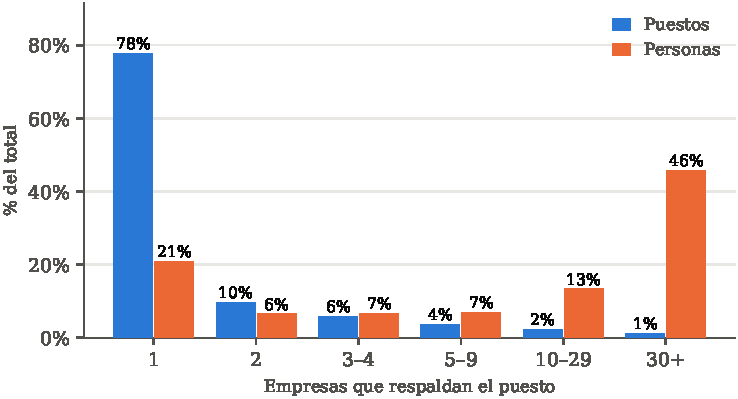
\includegraphics[width=\linewidth]{espesor_catalogo.pdf}
\caption[Espesor del catalogo de cargos]{\textbf{Casi todos los puestos son
delgados; casi toda la gente esta en los gruesos.} El 78\,\% de los 50.420 puestos
tiene una sola empresa detras y entre todos cubren el 21\,\% de las personas. En el
otro extremo, el 1\,\% de los puestos con 30 o mas empresas cubre el 46\,\%. Esa
asimetria es el problema: la cola larga no se arregla con mas modelo, se arregla
tomando fuerza prestada de un vecindario.}
\label{fig:espesor}
\end{figure}

La mitad de los titulos aparece en una sola empresa. Un tercio de las personas
esta en celdas de una o dos empresas. Calcular una mediana de mercado sobre eso
no da un benchmark: da el sueldo de un vecino.

Y el catalogo esta ademas sucio de una forma especifica. El mismo puesto aparece
tecleado de varias maneras ---seis variantes de espaciado de \cargo{ASISTENTE
ADMINISTRATIVO}, trece grafias de \cargo{VENDEDOR} incluyendo \cargo{VEENDEDOR},
\cargo{VENDEDRO} y \cargo{VEDEDOR}--- y cada una es, para el sistema, un puesto
distinto y delgado.

\section{El limite que ningun metodo basado en el puesto puede cruzar}

Antes de proponer nada conviene saber cuanto hay que ganar. Descomponiendo la
varianza del logaritmo del sueldo normalizado por el salario basico unificado,
dentro de cada celda de cargo:

\begin{equation}
y_{fi} = \mu_c + u_f + e_{fi}, \qquad
u_f \sim (0, \tau^2), \qquad
e_{fi} \sim (0, \sigma^2)
\label{eq:modelo}
\end{equation}

donde $f$ indexa empresas e $i$ personas dentro de la empresa. Medido sobre el
conjunto de ajuste:

\[
\tau = 0{,}2917 \qquad \sigma = 0{,}1423
\]

El efecto empleador $\tau$ es el doble que la dispersion dentro de la nomina.
\textbf{La empresa explica el 81\,\% de lo que no se puede predecir desde el
puesto.} Dos personas con el mismo cargo en empresas distintas cobran muy
diferente, y eso no es ruido de medicion: es la variable que de verdad gobierna
el salario y que un benchmark por puesto no puede ver.

De ahi sale el presupuesto del trabajo (figura~\ref{fig:descomposicion}). Comparando
la desviacion del error real contra el suelo irreducible:

\begin{table}[h]
\centering
\caption{Techo de mejora por agrupar mejor}
\begin{tabular}{lrrr}
\toprule
Subconjunto & sd real & sd irreducible & Techo \\
\midrule
Todo el ajuste & 0,3700 & 0,3253 & 12,1\,\% \\
Lejos del piso del SBU ($y > 0{,}05$) & 0,4322 & 0,3750 & 13,2\,\% \\
\bottomrule
\end{tabular}

\vspace{0.6ex}
{\footnotesize La misma descomposicion sobre la particion de evaluacion da
10,9\,\%. Las dos cifras son el mismo calculo con distinto alcance y conviene
citarlas por separado.}
\end{table}

\begin{figure}[htbp]
\centering
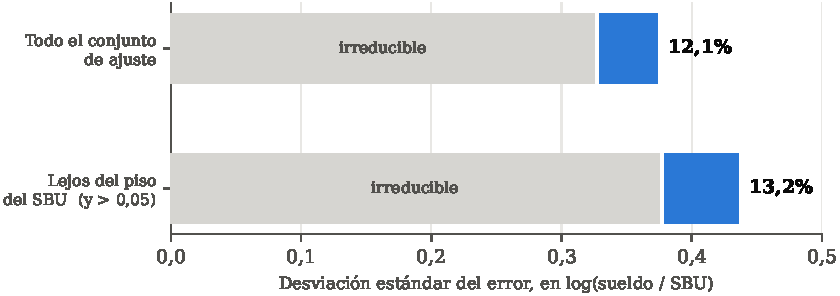
\includegraphics[width=\linewidth]{descomposicion_error.pdf}
\caption[Descomposicion del error de prediccion]{\textbf{La franja en color es todo
lo que una agrupacion mejor puede recuperar.} El resto lo genera el empleador:
$\tau = 0{,}29$ entre empresas frente a $\sigma = 0{,}14$ dentro de la nomina.
Cuanto mas lejos del piso del salario basico, mas margen hay ---abajo la
distribucion esta comprimida contra el minimo legal.}
\label{fig:descomposicion}
\end{figure}

\textbf{El techo es del orden del 12\,\%.} Cualquier resultado debe leerse contra
ese numero, no contra cero. Un metodo que reduzca el error un 4\,\% esta
recuperando un tercio de todo lo que habia disponible; uno que prometa un 40\,\%
esta midiendo mal.

Esta cifra es, en si misma, una contribucion: los trabajos previos comparan
metodos entre si sin establecer contra que techo compiten.

% ============================================================================
\chapter{Un resultado negativo en el centro}

\section{La premisa con la que arranco el proyecto}

El proyecto se diseno sobre la hipotesis de que la \textbf{composicion del pago}
---que fraccion del ingreso es sueldo fijo, comision, horas extra--- discrimina
puestos que la etiqueta confunde. La intuicion es razonable: un vendedor a
comision y un vendedor a sueldo hacen trabajos distintos aunque se llamen igual.

Sobre esa hipotesis se construyeron trece semanas de arquitectura: transformacion
ILR y aparato composicional, compuerta de masa fija, ponderacion por
probabilidad inversa, restricciones semi-supervisadas.

\section{Por que no se habia medido}

La composicion estaba disponible en el \textbf{2,7\,\%} de las filas. La hipotesis
se adopto \emph{por eliminacion} ---se descartaron sector, tamano y antiguedad, y
quedo ella--- y como el dato no estaba, \textbf{era infalsable en el momento de
adoptarla}.

Se recupero al 80\,\% arreglando el pipeline de ingesta (\dref{001}, \dref{008}),
se midio que es un rasgo estable entre anos, se midio cuanto de ella explica el
empleador. Nunca se midio lo unico que sostenia la tesis.

El hueco lo detecto una pregunta del director del proyecto: \emph{``sacamos la
composicion pero en el EDA nunca analizamos nada de eso para ver si efectivamente
es relevante''}.

\section{Lo que salio al medirlo}

\begin{table}[h]
\centering
\caption{Poder discriminante de cada eje candidato, fuera de muestra}
\label{tab:ejes}
\begin{tabular}{lrr}
\toprule
Eje & $R^2$ fuera de muestra & Reduce la sd \\
\midrule
Placebo & $-0{,}0002$ & --- \\
\textbf{Composicion del pago} & $+0{,}0042$ & 0,21\,\% \\
Antiguedad & $+0{,}0114$ & 0,57\,\% \\
\textbf{Rango jerarquico} ($\omega^2$, dentro de area) & $\mathbf{+0{,}2462}$ & \textbf{13,2\,\%} \\
\bottomrule
\end{tabular}
\end{table}

La composicion vale \textbf{0,21\,\% de reduccion de desviacion} sobre un techo
del 12\,\%, con un placebo en cero. El rango jerarquico vale \textbf{59 veces
mas}.

La afirmacion se enuncia estrecha, porque la medicion es estrecha: \emph{la
composicion no aporta informacion intra-empresa e intra-etiqueta sobre el sueldo
base}. No ``la composicion no importa'' --- sobre compensacion total es
mecanicamente casi todo, y el diseno residualiza contra la empresa, que determina
entre el 39\,\% y el 50\,\% de la propia composicion.

\section{El eje que si paga}

El rango jerarquico da una escalera monotona de cinco escalones (figura~\ref{fig:escalera})
con un recorrido de \textbf{$2{,}11\times$ en salario} entre el nivel 1 y el nivel 5. Se obtiene de
tres fuentes por orden de confianza:

\begin{enumerate}[nosep]
  \item \textbf{Lexico de rango} --- la palabra de jerarquia en el propio titulo
        (\cargo{AUXILIAR}, \cargo{ASISTENTE}, \cargo{JEFE}, \cargo{GERENTE}).
        Cubre el 34,5\,\% de las personas, es gratis y es auditable.
  \item \textbf{Catalogo MDT-2019-395}, niveles A--E oficiales definidos
        \emph{por contenido de puesto}, no por sueldo.
  \item Un clasificador para el resto, validado contra el 34,5\,\% donde la
        verdad se conoce.
\end{enumerate}

Que el catalogo oficial defina los niveles por contenido y no por remuneracion es
lo que permite usarlo sin circularidad.

\begin{figure}[htbp]
\centering
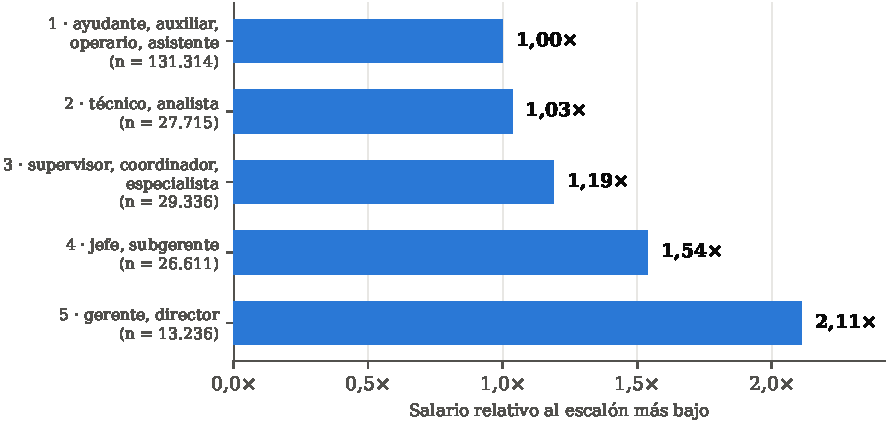
\includegraphics[width=\linewidth]{escalera_niveles.pdf}
\caption[Escalera salarial por escalon jerarquico]{\textbf{El eje que si paga.}
Efecto de cada escalon sobre el salario, \emph{dentro} de empresa y de area ---o sea
ya descontado el empleador, que es el factor dominante. La escalera es monotona y el
recorrido entre el escalon mas bajo y el mas alto es de $2{,}11\times$. Comparese con
la composicion del pago, que en la misma medicion vale un 0,21\,\% de reduccion de
desviacion (tabla~\ref{tab:ejes}).}
\label{fig:escalera}
\end{figure}

\section{La ceguera jerarquica de los embeddings}

El hallazgo que obliga a tratar el nivel aparte: el modelo de embeddings
multilingue codifica el \emph{area} del puesto y no su \emph{jerarquia}. Medido
sobre pares del catalogo:

\begin{table}[h]
\centering
\begin{tabular}{lr}
\toprule
Pares que difieren solo en el \textbf{rango} & coseno 0,857 \\
Pares que difieren solo en el \textbf{area} & coseno 0,764 \\
\bottomrule
\end{tabular}
\end{table}

El modelo considera \emph{mas parecidos} a dos puestos que difieren en jerarquia
que a dos que difieren en area. Como el nivel vale un recorrido de
$2{,}11\times$ en pago y el area no, agrupar por similitud semantica sin corregir
fusiona puestos que cobran el doble. La jerarquia tiene que entrar por otra via.

\section{La reformulacion}

El enunciado de la tesis pasa a ser:

\begin{quote}
\emph{¿Cuanto error de un benchmark salarial es reducible por elegir mejor el
grupo de comparacion, y que precision cuesta la taxonomia dura que vende la
industria?}
\end{quote}

Con ese enunciado el resultado modesto deja de ser una decepcion y pasa a ser una
medicion dentro de un presupuesto cuantificado. Y un modelo simple pasa a ser una
virtud metodologica: uno complicado confundiria el techo con la capacidad del
metodo.

\section{La leccion de proceso}

Una hipotesis que no se puede falsar con los datos que hay no es un cimiento: es
una apuesta. El correctivo no es desconfiar mas, sino \textbf{ordenar el trabajo
para que la premisa se mida primero}, aunque medirla exija arreglar el pipeline
antes.

De esta entrada sale ademas una regla operativa del repositorio: \emph{un numero
que no se puede reproducir no se defiende}. Toda medicion que sostenga una
afirmacion vive en \texttt{research/experimentos/} con su script y su salida,
commiteados el mismo dia en que se mide.

% ============================================================================
\chapter{El metodo}

\section{Vista general}

El sistema construye una \textbf{base de referencia} una vez y la consulta muchas.
Dado un titulo de puesto:

\begin{itemize}[nosep]
  \item si el titulo esta en la base, se usa la referencia de su propia celda;
  \item si es nuevo, se embebe y se coloca entre los puestos que se le parecen.
\end{itemize}

Lo segundo no es un adorno: \textbf{el 35,9\,\% de las personas de una nomina
nueva tiene un titulo que no esta en la base}. Sin la rama de analogia la
cobertura se queda en dos tercios.

El sistema \emph{siempre} responde. La decision es de producto: un cliente sin
referencia no se queda quieto, se inventa un numero. Pero como se responde
siempre, la marca de confianza deja de ser decorativa --- es lo unico que separa
``esto lo se'' de ``esto lo estoy suponiendo''.

\section{El estimador: pesos inverso-varianza}

Del modelo de la ecuacion~\eqref{eq:modelo} se deriva todo lo demas sin
hiperparametros. El voto de cada empresa $f$ en una celda es la mediana de sus
personas, $m_f$, y se pondera por

\begin{equation}
w_f = \frac{1}{\tau^2 + \sigma^2 / n_f}
\label{eq:peso}
\end{equation}

La referencia es el cuantil ponderado al 50\,\% de los votos $\{m_f\}$ con esos
pesos.

Este peso resuelve un debate de diseno que antes se zanjaba por criterio. Sus dos
regimenes limite son las dos posturas:

\begin{table}[h]
\centering
\begin{tabular}{lll}
\toprule
Regimen & $w_f$ tiende a & Equivale a \\
\midrule
$n_f \to \infty$ & $1/\tau^2$, igual para todas & una empresa, un voto \\
$\tau^2 \to 0$ & $n_f/\sigma^2$ & una persona, un voto \\
\bottomrule
\end{tabular}
\end{table}

Y lo que resuelve el problema practico: \textbf{el ratio maximo entre pesos esta
acotado por $1 + \sigma^2/\tau^2 \approx 1{,}24$}, no por el tamano relativo de
las empresas. Una empresa de 3.000 personas no puede dominar la celda, y no hace
falta descartar el voto de las pequenas para conseguirlo.

Esta estructura ancla el trabajo en estimacion en areas pequenas ---tomar fuerza
prestada de un vecindario--- y no en la busqueda de una variable que faltaba.

\section{El vecindario semantico y por que no se pesa por similitud}

Para un titulo nuevo hay que combinar las celdas vecinas. La version ingenua pesa
cada vecino por \emph{similitud} $\times$ \emph{precision}. Medido sobre un caso
real, eso rompe:

\begin{table}[h]
\centering
\caption{Por que la ponderacion ingenua falla: \cargo{OPERADOR DE PARQUEADERO}}
\begin{tabular}{lrr}
\toprule
Vecino & Similitud & Peso ingenuo \\
\midrule
\cargo{OPERADOR DE PARQUEADEROS} & 0,989 & 8\,\% \\
\cargo{OPERADOR DE EXCAVADORA} & 0,825 & \textbf{46\,\%} \\
\bottomrule
\end{tabular}
\end{table}

El sistema tenia la respuesta exacta delante y le hizo caso a una excavadora,
porque la excavadora tenia mas datos. La correccion es tratar cada vecino como
una \emph{observacion ruidosa} del puesto objetivo, con varianza

\begin{equation}
\mathrm{var}_j = \underbrace{1/W_j}_{\text{error de medicion}} +
                 \underbrace{\lambda\,(1 - s_j)}_{\text{castigo por no ser el mismo puesto}}
\label{eq:varvecino}
\end{equation}

y pesar por $1/\mathrm{var}_j$. Un vecino lejano se descuenta aunque este
perfectamente medido.

\textbf{$\lambda$ se estima de los datos, no se elige}: es cuanto difieren de
verdad dos celdas por unidad de distancia semantica. Se estima por escalon
jerarquico, porque varia un factor 18 entre ellos.

Esta formulacion resuelve sola el caso degenerado. Para \cargo{LOTERO} el
embedding no encuentra nada parecido y se agarra a la terminacion \emph{-ero}:
\cargo{LINIERO}, \cargo{BOTERO}, \cargo{LAMPERO}, \cargo{TESORERO}, todos entre
0,748 y 0,784 de similitud. \cargo{TESORERO} paga 2,5 veces mas. Con la varianza
de la ecuacion~\eqref{eq:varvecino}, si todos los vecinos estan lejos el termino
$\lambda(1-s_j)$ domina, el intervalo se dispara y la confianza cae a BAJA sin
que haya que programar ninguna excepcion.

\section{Consolidacion de grafias}

Antes de estimar nada, las grafias del mismo puesto se juntan. Tres pasadas, en
orden y por separado para que cada una sea auditable:

\begin{enumerate}[nosep]
  \item \textbf{Semantica}, por enlace completo sobre el grafo de similitud con
        umbral 0,95. El enlace \emph{completo} y no el simple: medido, el enlace
        simple percola --- produce un grupo de 1.758 titulos que contiene a la vez
        \cargo{ASISTENTE CONTABLE} y \cargo{AUXILIAR DE LIMPIEZA}, unidos por una
        cadena de saltos individualmente razonables.
  \item \textbf{Por errata}, con indexado por variantes de borrado. Absorbe el
        grupo raro dentro del comun exigiendo asimetria: el lado raro con
        $\le 2$ empresas, el comun con $\ge 10$.
  \item \textbf{Por grafia de genero}, que unifica \cargo{ENFERMERA} y
        \cargo{ENFERMERO} conservando y reportando la diferencia que habia antes
        de unirlos.
\end{enumerate}

La fusion sube la cobertura directa del \textbf{57,7\,\% al 64,1\,\%} sin costar
precision.

Un hallazgo lateral vale la pena: \textbf{el embedding no reconoce una errata de
una letra}. \cargo{VENDEROR} contra \cargo{VENDEDOR} puntua 0,7177 frente a un
umbral de fusion de 0,95. Las trece grafias de vendedor las unio la regla
ortografica, no el modelo semantico.

\section{La banda}

El entregable no es un numero sino un intervalo, y la pregunta que responde es
\emph{que paga la mitad central de las empresas}. De ahi dos decisiones:

\begin{itemize}[nosep]
  \item \textbf{$\sigma$ no entra en la banda de empresas.} El nivel de una
        empresa es $\mu_c + u_f$, con varianza $\tau_c^2$; $\sigma^2$ separa a dos
        personas de la misma nomina y no mueve el nivel del empleador.
  \item \textbf{Con datos de sobra se usan los cuantiles empiricos} de los votos,
        no una normal. Describen la forma real, que va de un pico a una cola larga
        segun el cargo.
\end{itemize}

Se entregan dos bandas: la de \emph{empresas} para decisiones de politica
salarial, y la de \emph{personas} ---que si lleva $\sigma$--- para situar a un
individuo.

\section{Correccion por tamano de empresa}

Segmentar el mercado por tamano \emph{no} estrecha la banda: medido, la
incertidumbre del centro sube mas de lo que baja el ancho. Pero el tamano si
corrige un \textbf{sesgo grande en el centro} de los cargos altos.

El caso que lo muestra: a una empresa pequena se le decia que su gerente general
cobra un 56\,\% por debajo del mercado, cuando entre sus pares de tamano estaba
bien. La correccion por desplazamiento lleva el rango de error de
$-56{,}0\,\%/+81{,}9\,\%$ a $-12{,}1\,\%/+17{,}9\,\%$.

La leccion metodologica es que \emph{segmentar para estrechar} y \emph{segmentar
para corregir el centro} son dos preguntas distintas y la respuesta no es la
misma.

% ============================================================================
\chapter{Protocolo de medicion}

El instrumento se construyo antes que el modelo, deliberadamente (\dref{002}). La
contribucion del trabajo es la medicion, no el algoritmo, y una regla de medicion
torcida no se detecta midiendo: se detecta auditandola antes de usarla.

\section{Las reglas}

\begin{description}[style=nextline,nosep]
  \item[Particion por empresa, nunca por fila.] El empleador explica el 39\,\% del
        salario. Con particion aleatoria por fila, la empresa de test aparece en
        train y se acierta por la razon equivocada.
  \item[Todo intervalo se remuestrea por empresa.] La fila no es la unidad
        independiente: una persona recurre entre anos y una empresa aporta cientos
        de personas. Tratarlas como independientes estrecha los intervalos sin
        derecho.
  \item[Puntuacion propia.] La perdida \emph{pinball} en $q = 0{,}25$ y
        $q = 0{,}75$ sobre la banda de empresas. Es estrictamente propia: se
        minimiza diciendo la verdad. El error absoluto es su caso degenerado.
  \item[Criterio escrito antes de mirar.] Cada experimento declara en su
        encabezado que resultado lo adoptaria y cual lo rechazaria, antes de
        correr.
  \item[Placebo en todo cambio de agrupacion.] Cualquier reagrupacion mejora la
        cobertura por construccion. El placebo ---mismos grupos, destinos
        barajados--- es lo unico que distingue senal de mecanica.
  \item[El 20\,\% de test no se toca] hasta que el metodo este congelado en el
        pre-registro.
\end{description}

\section{Por que el placebo es la pieza que decide}

Tres ejemplos de esta misma serie de experimentos:

\begin{itemize}[nosep]
  \item En la fusion por errata (\dref{025}) el placebo \emph{no} tuvo potencia, y
        la decision se registro como ``no validada, solo no contradicha''.
  \item Al ampliar esa regla (\dref{031}) el placebo si discrimino: mandar las
        mismas absorciones a destinos al azar cuesta $+0{,}00130$ de pinball
        frente a $-0{,}00001$ de la regla real, cien veces mas. Eso es lo que
        demuestra que la distancia de edicion elige bien el destino.
  \item En la segmentacion selectiva por tamano (\dref{018}) el placebo
        \textbf{eligio mas cargos que la seleccion real} --- 118 contra 93 --- lo
        que basto para descartar el metodo.
\end{itemize}

% ============================================================================
\chapter{Lo que se midio y no entro}

Un catalogo de resultados negativos no es un apendice: es lo que impide que el
lector suponga que lo obvio no se probo.

\begin{table}[h]
\centering
\caption{Hipotesis medidas y rechazadas}
\label{tab:negativos}
\small
\begin{tabular}{p{4.2cm}p{6.5cm}l}
\toprule
Hipotesis & Resultado & Ref. \\
\midrule
La composicion del pago discrimina puestos &
$R^2 = +0{,}0042$ contra placebo $-0{,}0002$. Vale 0,21\,\% sobre un techo del 12\,\% &
\dref{013} \\[0.8ex]

El sector estrecha la banda &
pinball $0{,}1289$ contra $0{,}1255$ sin segmentar. Empeora &
\dref{022} \\[0.8ex]

El sector corrige el centro &
No se sostiene fuera de muestra. Se retira lo adoptado en \dref{014} &
\dref{022} \\[0.8ex]

La escalera de niveles debe estimarse con medianas &
La mediana pierda contra la media: $+0{,}00069$, IC sobre cero. Hipotesis propia rechazada &
\dref{024} \\[0.8ex]

Comparar contra el sector especifico del cliente (division o clase CIIU) &
Peor cuanto mas fino. Cambia el veredicto del 1,79\,\% de los cargos y en esos la seccion acierta un 9,2\,\% mas &
\dref{029} \\[0.8ex]

Dar contexto al embedding mejora la representacion &
Mejora el vecindario (2/5 a 4/5 en pares sinonimo/rima) y \emph{no} mueve las bandas: IC cruza el cero &
\dref{030} \\[0.8ex]

Excluir al cliente de su propio mercado &
Quitar una empresa mueve el centro un 1,2\,\% de la barra de error ya declarada. Corregirlo seria corregir ruido &
\dref{027} \\
\bottomrule
\end{tabular}
\end{table}

\section{El caso del sector, que se adopto y luego se retiro}

Merece detalle porque es el unico eje que entro al modelo y despues salio.

\dref{014} lo adopto como ``segundo eje del arquetipo'' con una reduccion del
13,2\,\% de desviacion dentro de las etiquetas anchas y un placebo en 0,9\,\%. La
condicion que se le puso fue medirlo \emph{fuera de muestra}. Al hacerlo
(\dref{022}) no se sostuvo, ni para la banda ni para el centro, y se retiro.

La razon de fondo aparecio despues, al descomponer la varianza: de la diferencia
de pago \emph{entre empresas} por un mismo cargo, la division CIIU explica
\textbf{6 puntos netos} --- $0{,}389$ en crudo contra $0{,}325$ barajando, o sea
que casi todo es inflacion mecanica de partir en grupos pequenos. Lo que una
empresa paga por un contador depende de la empresa, no de si vende libros o
repuestos.

El sector permanece en el producto como \emph{lente} ---el cliente ve contra que
sector se le compara--- pero no como mejora del modelo, y eso esta escrito donde
se implementa.

% ============================================================================
\chapter{Resultados}

\section{Cobertura}

\begin{table}[h]
\centering
\caption{Cobertura del benchmark}
\begin{tabular}{lr}
\toprule
Techo de cobertura de la etiqueta cruda & 66,6\,\% \\
Cobertura directa antes de consolidar grafias & 57,7\,\% \\
Cobertura directa despues de consolidar & \textbf{64,1\,\%} \\
Personas de una nomina nueva con titulo desconocido & 35,9\,\% \\
\bottomrule
\end{tabular}
\end{table}

La rama de analogia es lo que convierte un sistema que cubre dos tercios en uno
que responde siempre. El coste de responder siempre se paga en la marca de
confianza, no en silencio.

\section{Estado del sistema}

\begin{table}[h]
\centering
\caption{El artefacto}
\begin{tabular}{lr}
\toprule
Titulos en la base & 65.181 \\
Puestos tras consolidar grafias & 50.420 \\
Empresas que aportan datos & 6.722 \\
Empresas resolubles por RUC (registro completo) & 221.754 \\
Decisiones de metodo registradas con evidencia & 31 \\
Pruebas automatizadas & 381 \\
\bottomrule
\end{tabular}
\end{table}

% ============================================================================
\chapter{Limitaciones}

\begin{description}[style=nextline]
  \item[El techo es el techo.] El empleador explica el 81\,\% de lo que no se
        puede predecir desde el puesto. Este trabajo entrega el \emph{mercado},
        no la politica salarial de una empresa concreta, y ningun metodo basado
        en la etiqueta de puesto puede cruzar esa frontera.

  \item[El conjunto de test sigue sin tocarse.] Todo lo reportado esta medido
        sobre particiones de validacion dentro del conjunto de ajuste. Es
        correcto por diseno ---el test se toca una vez, despues del
        pre-registro--- pero significa que lo que hay es consistencia interna,
        no generalizacion demostrada.

  \item[Dos anos de datos.] El universo es 2024--2025, los unicos anos con
        plantilla completa. No hay serie temporal suficiente para separar
        tendencia de nivel.

  \item[El 30\,\% de las empresas no cruza con el registro.] De las 6.722 que
        aportan datos, 1.987 no presentan balances en la Superintendencia
        ---probablemente sector publico, fundaciones y personas naturales--- y
        para ellas no hay sector ni tamano.

  \item[El modelo de embeddings es un limite blando.] Con titulos de una a tres
        palabras en espanol no separa el sinonimo de la rima: \cargo{DENTISTA}
        puntua 0,752 con \cargo{TELEFONISTA} y 0,763 con \cargo{ODONTOLOGA}.
        Once milesimas entre una terminacion compartida y un sinonimo. Medido
        (\dref{030}), esto degrada el buscador de puestos y \emph{no} degrada las
        bandas, porque la banda depende de cuantas empresas respaldan el cargo
        mucho mas que de cual es su vecino mas cercano.
\end{description}

% ============================================================================
\chapter{Conclusiones}

\begin{enumerate}
  \item \textbf{El presupuesto esta cuantificado.} El techo de mejora por
        agrupar mejor es del orden del 12\,\%, y el 81\,\% de lo irreducible lo
        genera el empleador. Cualquier afirmacion sobre benchmarking salarial
        deberia declarar contra que techo compite.

  \item \textbf{La premisa central del proyecto era falsa y se midio.} La
        composicion del pago vale 0,21\,\% de reduccion de desviacion contra un
        placebo en cero. El eje que paga es el nivel jerarquico, con
        $\omega^2 = 0{,}2462$ y un recorrido de $2{,}11\times$.

  \item \textbf{El problema es de estimacion en areas pequenas}, no de encontrar
        la variable que faltaba. La etiqueta de cargo no esta semanticamente
        rota: esta estadisticamente delgada, con mediana de dos personas y una
        empresa por titulo.

  \item \textbf{Los embeddings son ciegos a la jerarquia} y eso no es un detalle:
        el eje al que son ciegos vale $2{,}11\times$ en pago y el que si capturan
        no. Agrupar por similitud semantica sin corregir fusiona puestos que
        cobran el doble.

  \item \textbf{El protocolo produjo mas hallazgos que el modelo.} De las 31
        decisiones registradas, siete son resultados negativos que cerraron
        lineas de trabajo, y tres de ellas contradijeron hipotesis propias
        (\dref{013}, \dref{022}, \dref{024}). El placebo y el criterio escrito
        antes de mirar son lo que hizo esos hallazgos visibles.
\end{enumerate}

% ============================================================================
\begin{thebibliography}{9}

\bibitem{fay1979}
Fay, R.~E. y Herriot, R.~A. (1979).
\emph{Estimates of income for small places: an application of James--Stein
procedures to census data}.
Journal of the American Statistical Association, 74(366), 269--277.
\hfill [VERIFICAR paginacion]

\bibitem{rao2015}
Rao, J.~N.~K. y Molina, I. (2015).
\emph{Small Area Estimation}, 2.\textsuperscript{a} ed.
Wiley.

\bibitem{gneiting2007}
Gneiting, T. y Raftery, A.~E. (2007).
\emph{Strictly proper scoring rules, prediction, and estimation}.
Journal of the American Statistical Association, 102(477), 359--378.
\hfill [VERIFICAR paginacion]

\bibitem{zaoui}
Zaoui, A., Denis, C. y Hebiri, M.
\emph{Regression with reject option and application to kNN}.
\hfill [VERIFICAR ano y venue]

\bibitem{mdt2019}
Ministerio del Trabajo del Ecuador (2019).
\emph{Acuerdo Ministerial MDT-2019-395}: escala de niveles ocupacionales.

\bibitem{mdt2025}
Ministerio del Trabajo del Ecuador (2025).
\emph{Acuerdo Ministerial MDT-2025-195}: salario basico unificado 2026.
Registro Oficial, Suplemento 187, 18 de diciembre de 2025.

\end{thebibliography}

\end{document}
